\documentclass[12pt]{beamer}
%\documentclass[20pt,handout]{beamer}
\usetheme{Darmstadt}
\usepackage{graphicx}
%\usepackage[german]{babel}
\usepackage{ngerman}
\usepackage[T1]{fontenc}
\usepackage[utf8]{inputenc}
\usepackage{tikz}
\setbeamertemplate{footline}[frame number]

\newcommand{\cc}[1]{\includegraphics[height=4mm]{img/#1.png}\hspace{1mm}}
\usepackage{ifthen}
\newcommand{\license}[2][]{\\#2\ifthenelse{\equal{#1}{}}{}{\\\scriptsize\url{#1}}}
\usepackage{textcomp}
\usepackage{hyperref}

\pgfdeclareimage[height=.6cm]{c3d2logo}{./img/c3d2.pdf}


\pgfdeclarelayer{foreground}
\pgfsetlayers{main,foreground}
\logo{\pgfputat{\pgfxy(-1,0)}{\pgfbox[center,base]{\pgfuseimage{c3d2logo}}}}


\title{2 Jahre Snowden}
\author{\small Stephan Thamm\\\large Chaos Computer Club Dresden}
\date{15.11.2015}

\begin{document}
\maketitle

\section{Einleitung}
\subsection{}

\begin{frame}
    \frametitle{Chaos Computer Club}
    \begin{center}
	
\includegraphics[height=0.2\textheight]{img/chaosknoten.png}
    \end{center}	
    \begin{itemize}
      \item<1-> Verein wurde 1981 gegr"undet (\url{https://ccc.de})          
      \item<2-> Aktuell ca. 4500 Mitglieder
      \item<3-> Betreibt u.a. "Offentlichkeitsarbeit und Politikberatung      
    \end{itemize}
\end{frame}

\begin{frame}
  \frametitle{Chaos Computer Club}
  \begin{figure}
    
\includegraphics[height=0.7\textheight]{img/fingerabdruck.jpg}
  \end{figure}
\end{frame}

\begin{frame}
  \frametitle{Chaos Computer Club}
  \begin{figure}
    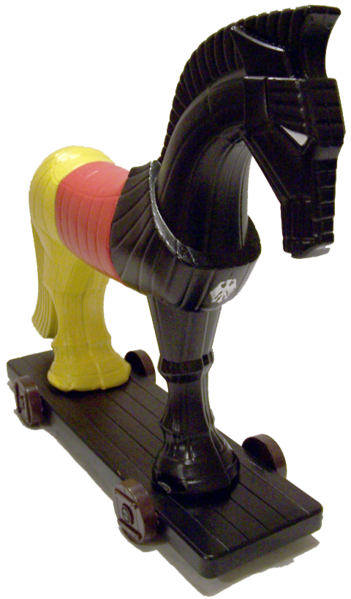
\includegraphics[height=0.7\textheight]{img/trojaner.png}
  \end{figure}
\end{frame}

\begin{frame}
    \frametitle{Chaos Computer Club}
    \begin{center}
	
\includegraphics[height=0.1\textheight]{img/c3d2_logo.png}
    \end{center}
    \begin{itemize}
      \item<1-> Chaos Computer Club Dresden (\url{https://c3d2.de})          
      \item<2-> Datenspuren (\url{https://datenspuren.de})
      \item<3-> Podcasts (\url{https://c3d2.de/radio.html})
      \item<4-> Chaos macht Schule (\url{https://c3d2.de/schule.html})
    \end{itemize}
\end{frame}

\section{Snowden Enthüllungen}
\subsection{}

\begin{frame}
    \frametitle{Bundespräsident Gauck zur NSA-Überwachung}
    \begin{center}
      ``Wir wissen z.B., dass es nicht so ist, wie bei der Stasi und dem KGB, dass es dicke Aktenbände gibt, wo unsere Gesprächsinhalte alle aufgeschrieben und schön abgeheftet sind. Das ist es nicht.''
      (Gauck, 30.06.2013 im ZDF-Sommerinterview)
    \end{center}
\end{frame}

\begin{frame}
    \frametitle{Stasi vs. NSA}
    \begin{center}
	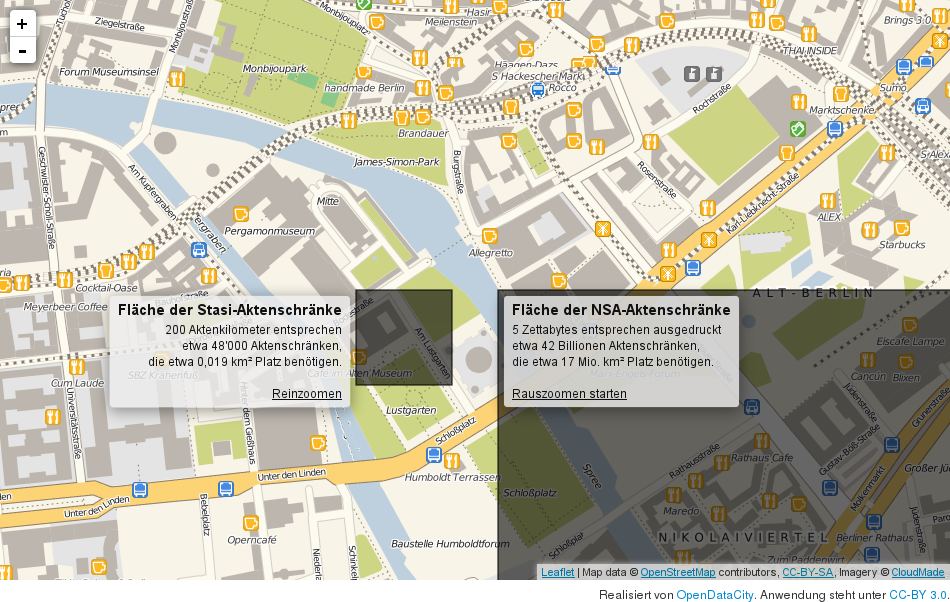
\includegraphics[height=0.7\textheight]{img/akten1.png}
    \end{center}
\end{frame}

\begin{frame}
    \frametitle{Stasi vs. NSA}
    \begin{center}
	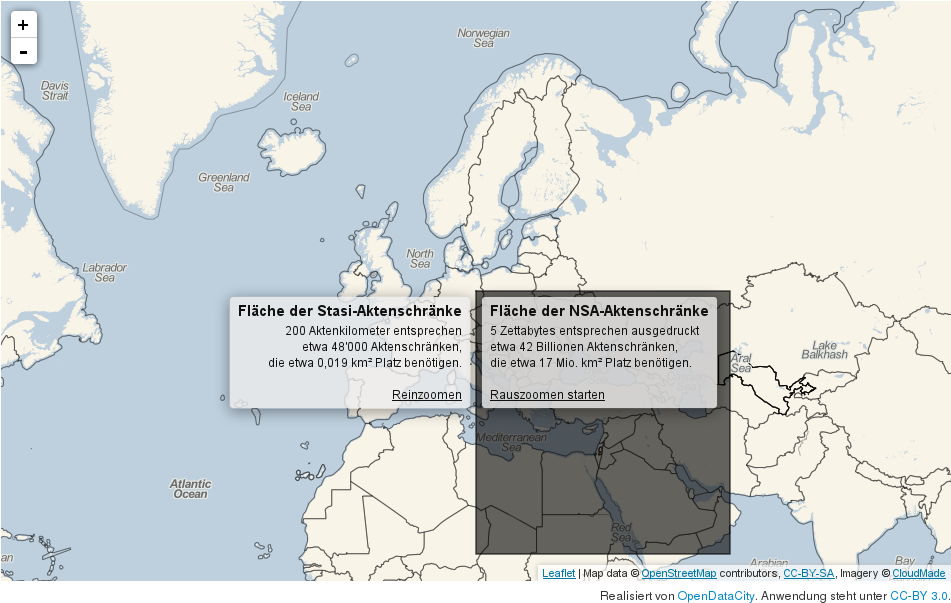
\includegraphics[height=0.7\textheight]{img/akten2.png}
    \end{center}
\end{frame}

\begin{frame}
    \frametitle{NSA-Skandal}
    \begin{center}
	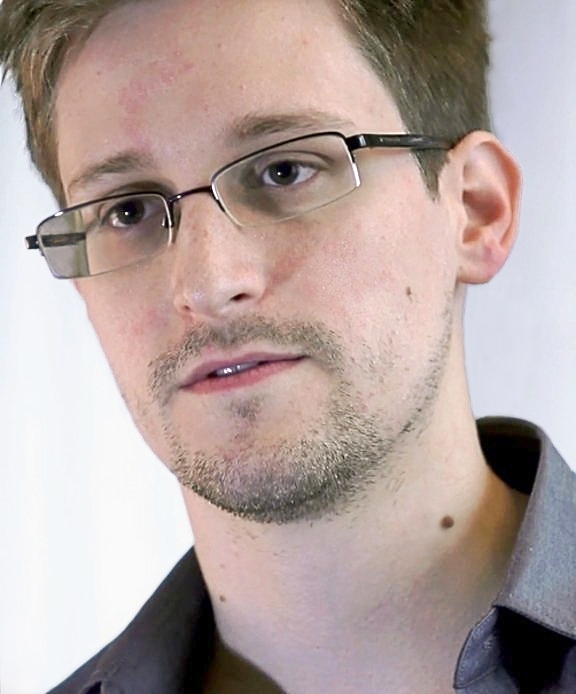
\includegraphics[height=0.7\textheight]{img/snowden.jpg}
	\\{\small \href{https://commons.wikimedia.org/wiki/File:Edward_Snowden.jpg\#mediaviewer/File:Edward_Snowden-2.jpg}{Grafik}: \href{https://creativecommons.org/licenses/by/3.0/}{\cc{by}} Laura Poitras / Praxis Films}
    \end{center}	
\end{frame}

\begin{frame}
  \frametitle{Tempora}
  \pause
  \begin{center}
    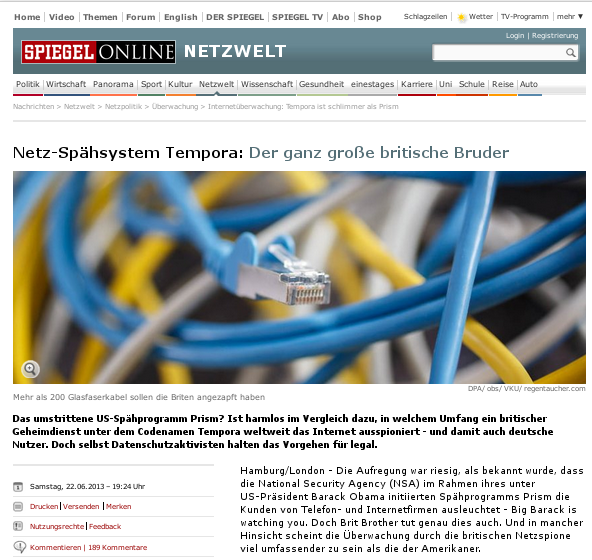
\includegraphics[height=0.7\textheight]{img/spiegel-tempora.png}
  \end{center}	
\end{frame}

\begin{frame}
  \frametitle{Prism}
  \pause
  \begin{center}
    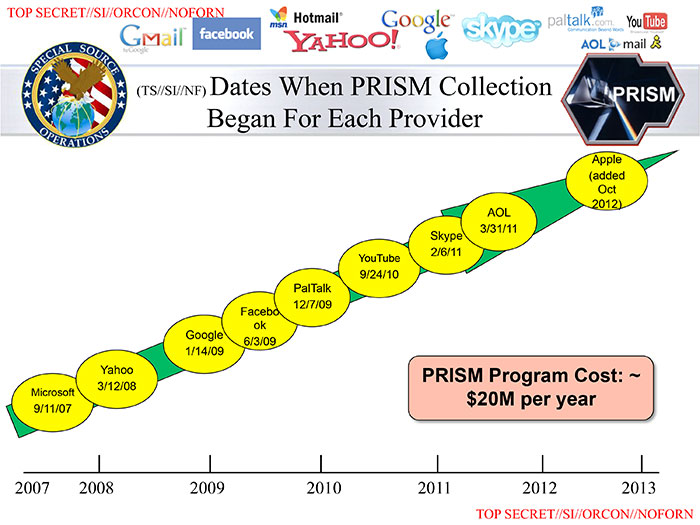
\includegraphics[height=0.7\textheight]{img/prism.jpg}
  \end{center}
\end{frame}

\section{Reaktionen}
\subsection{}

\begin{frame}
  \frametitle{USA}
  \pause
  \begin{center}
    \huge Landesverrat
  \end{center}
\end{frame}

\begin{frame}
  \frametitle{Firmen}
  \pause
    \begin{center}
      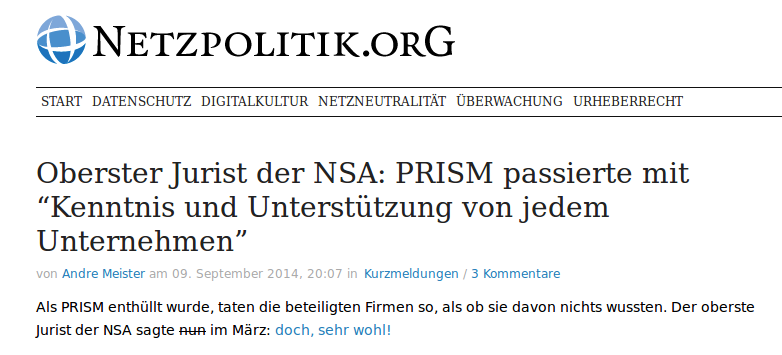
\includegraphics[height=5cm]{img/prism_netzpolitik.png}
    \end{center}
\end{frame}

\begin{frame}
  \frametitle{Deutschland}
  \pause
    \begin{center}
      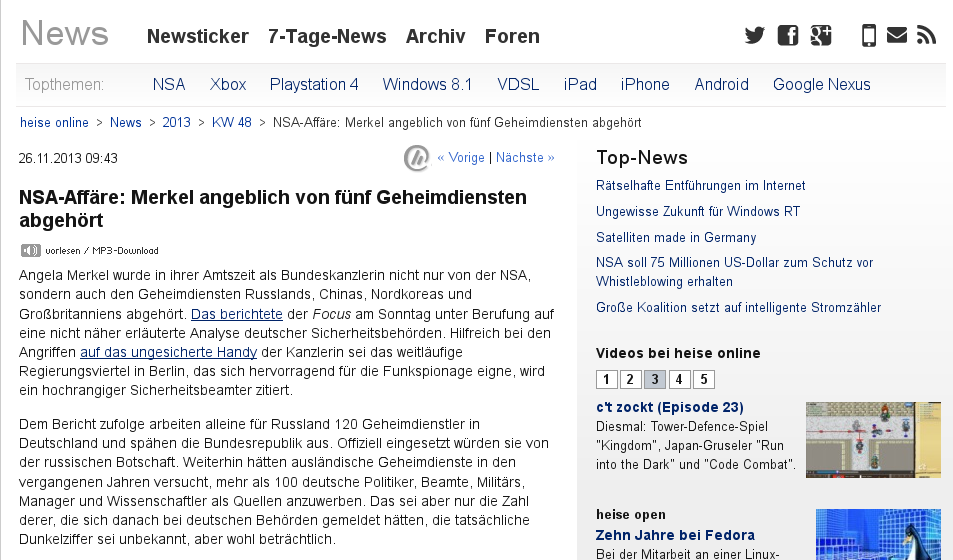
\includegraphics[height=5cm]{img/heise-merkel.png}
    \end{center}
\end{frame}

\begin{frame}
  \frametitle{Untersuchungsausschuss}
  \pause
    \begin{center}
      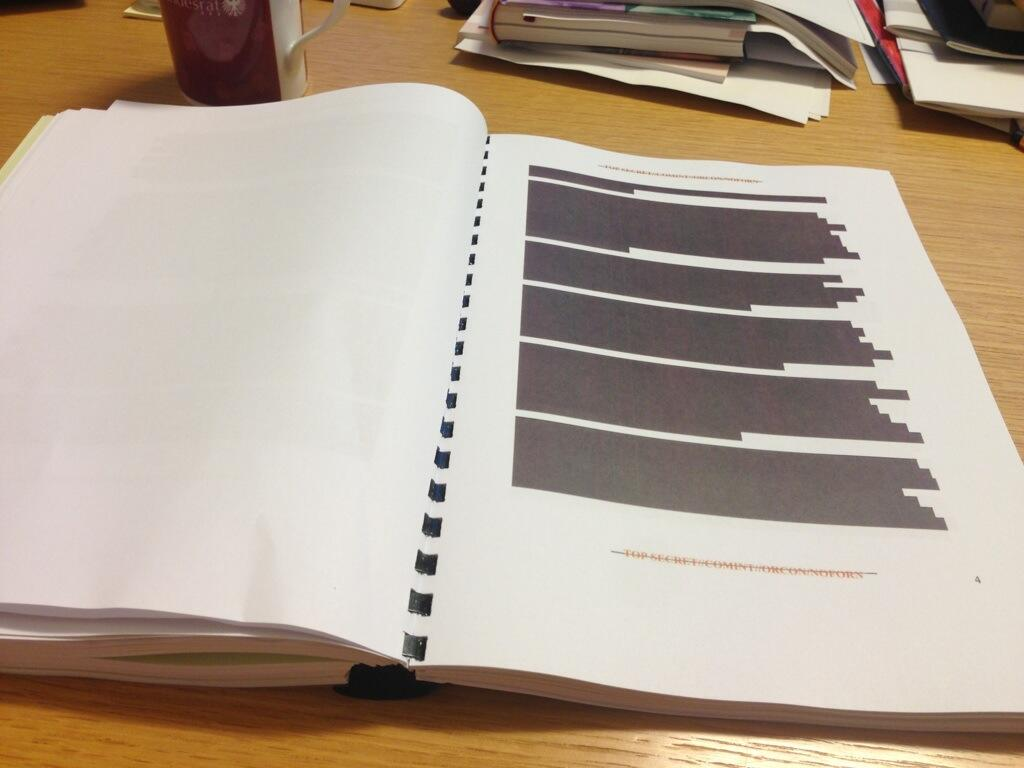
\includegraphics[height=5cm]{img/nsa-ua-akte.jpg}
    \end{center}
\end{frame}

\section{Aktuelle Entwicklungen}
\subsection{}

\begin{frame}
  \frametitle{EU-Datenschutzgesetz}
    \begin{center}
      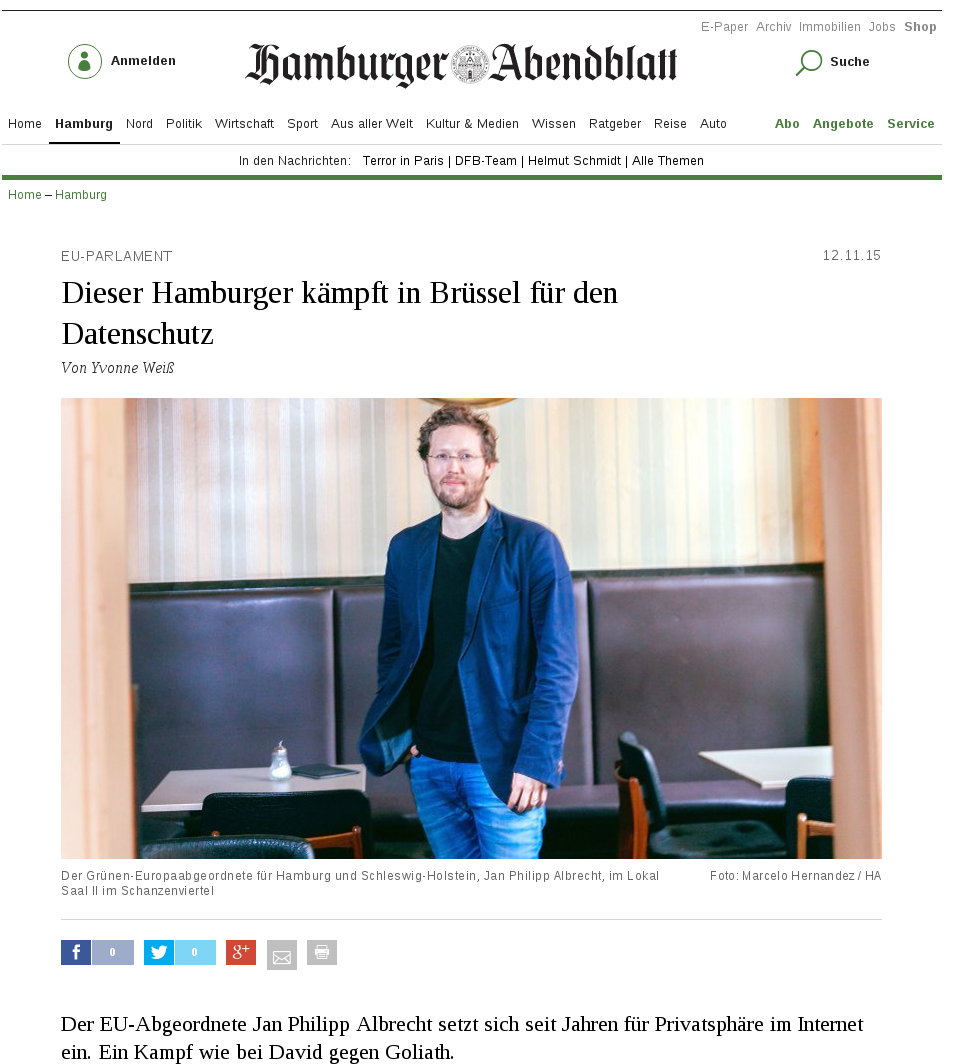
\includegraphics[height=5cm]{img/datenschutz-eu.png}
    \end{center}
\end{frame}

\begin{frame}
  \frametitle{Vorratsdatenspeicherung}
    \begin{center}
      \only<2>{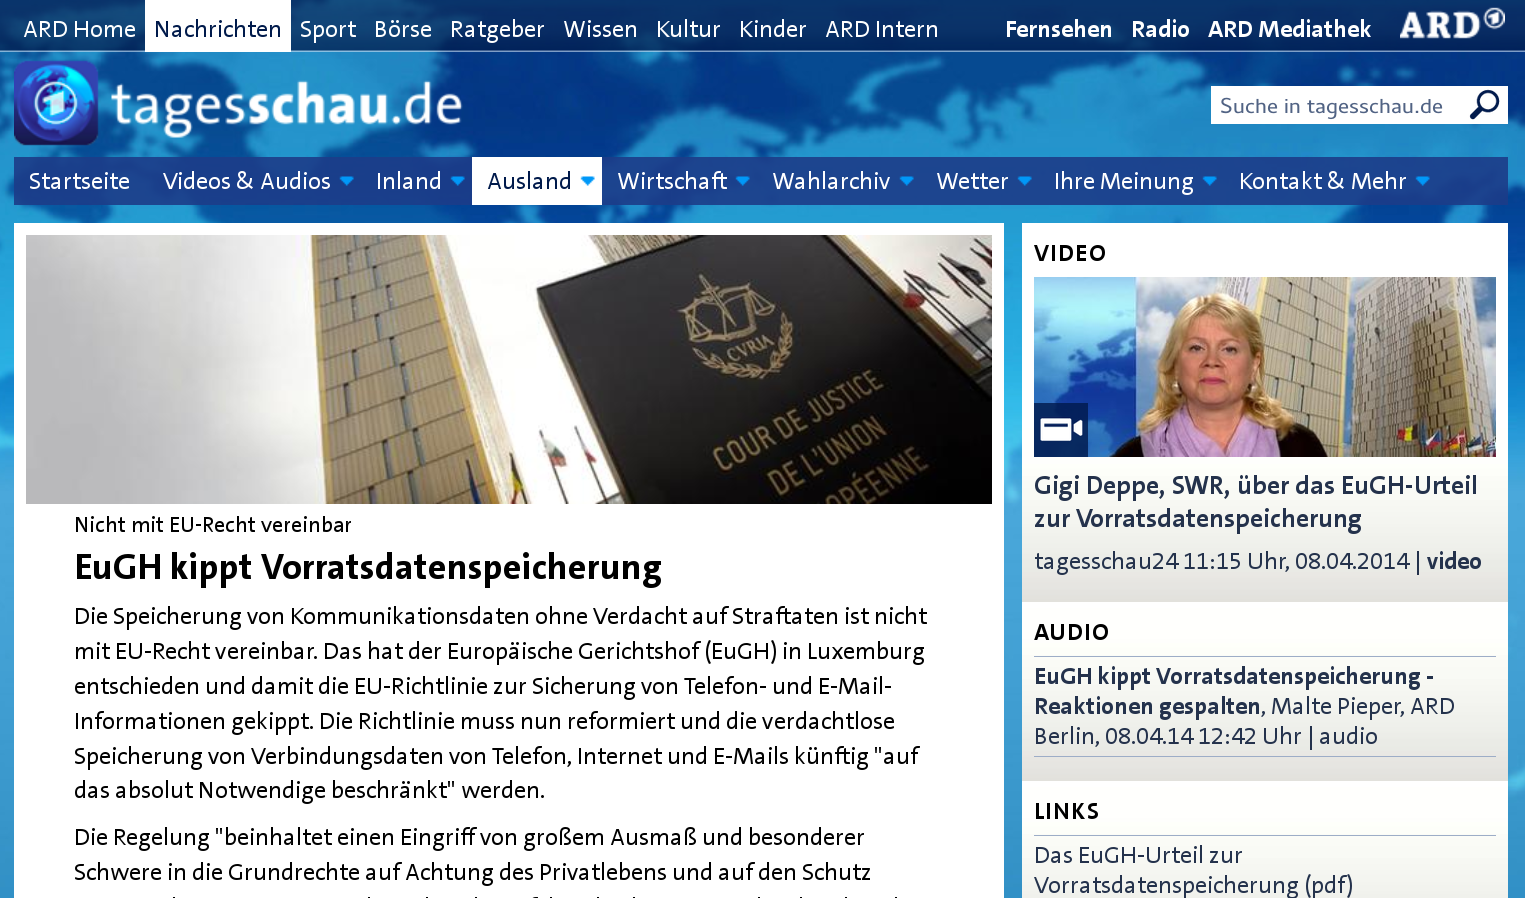
\includegraphics[height=5cm]{img/tagesschau-vds.png}}
      \only<3>{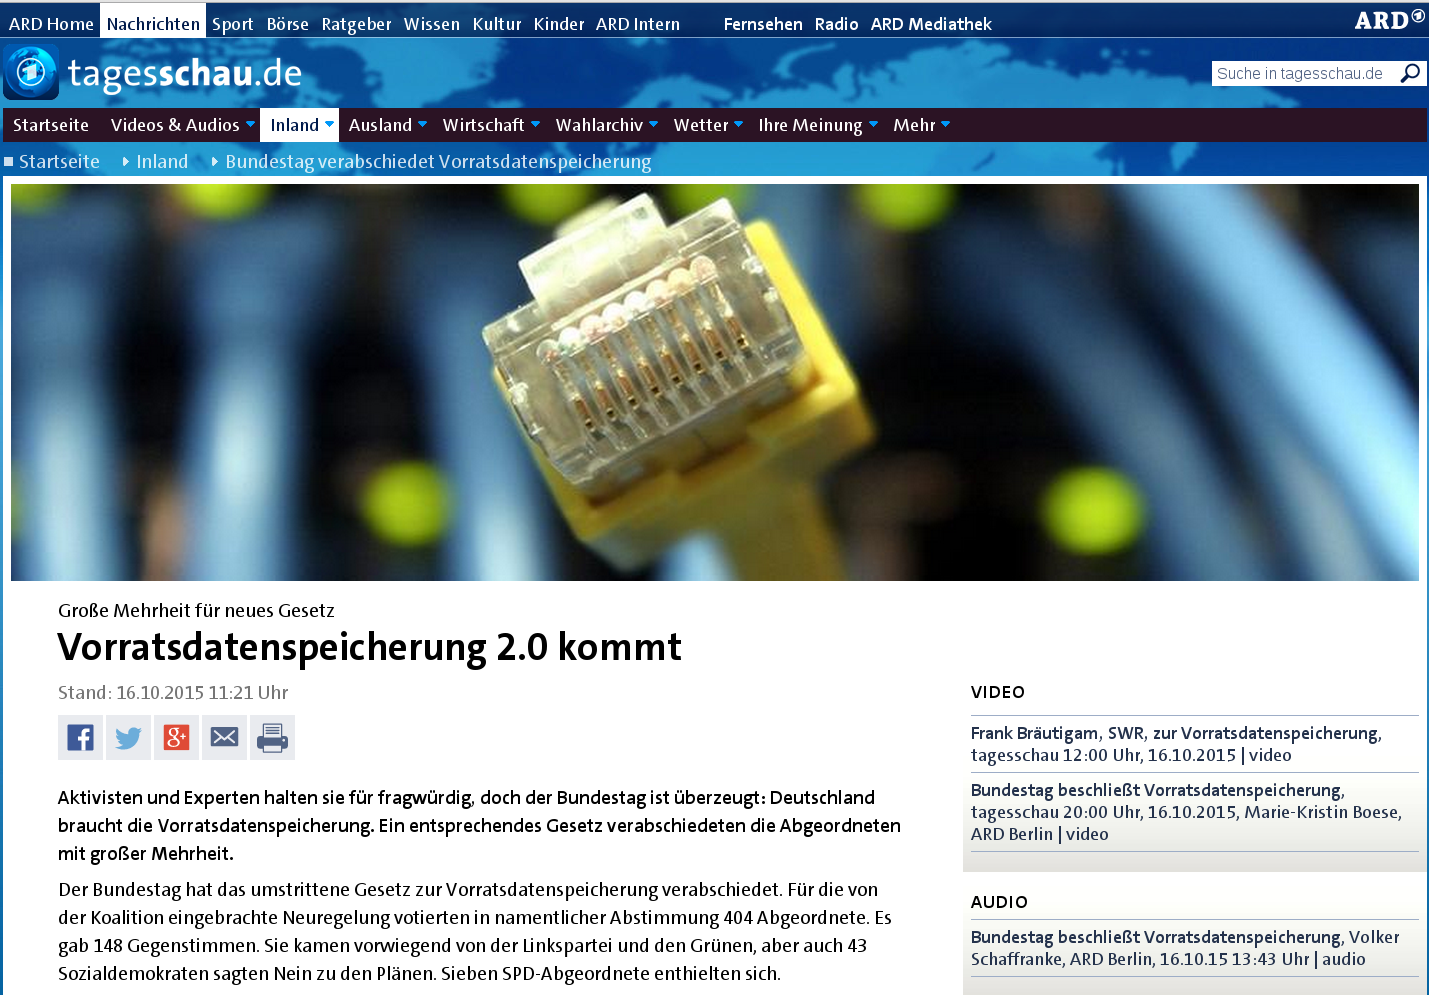
\includegraphics[height=5cm]{img/tagesschau-vds-2.png}}
    \end{center}
\end{frame}

\begin{frame}
  \frametitle{Metadaten}
  \begin{itemize}
    \item Handynetz
      \begin{itemize}
        \item Telefonnummern
        \item Zeitpunkt und Dauer (Telefonate, SMS)
        \item Funkzelle (Ort)
      \end{itemize}
    \item Internet
      \begin{itemize}
        \item IP-Adresse
        \item Alle Verbindungen
        \item Email: Adressen von Sender und Empfänger, Zugriff
      \end{itemize}
  \end{itemize}
\end{frame}

\begin{frame}
    \frametitle{Metadaten}
    \begin{center}
	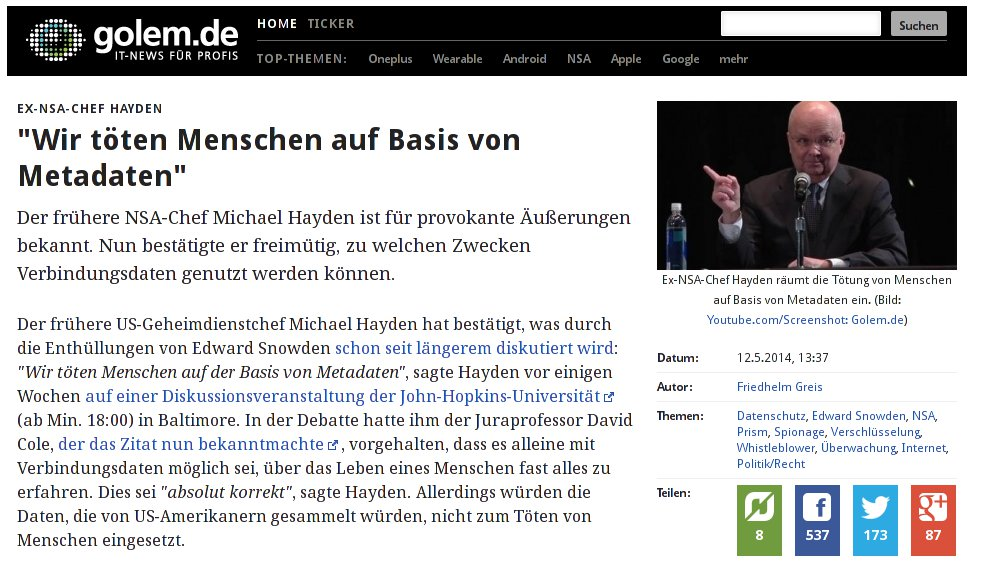
\includegraphics[height=0.7\textheight]{img/wekillpeople.jpg}
    \end{center}
\end{frame}

\begin{frame}
  \frametitle{Landesverrat}
  \begin{center}
    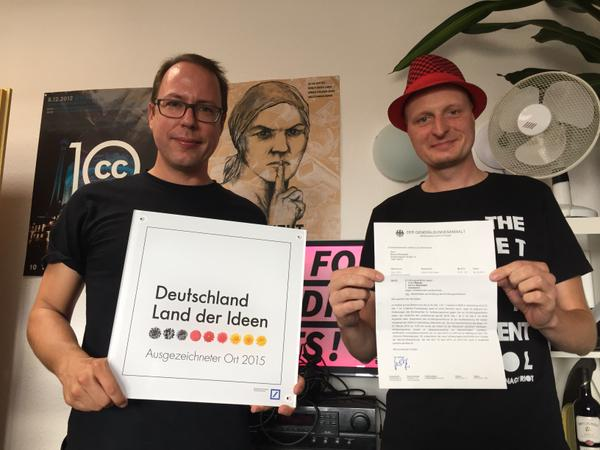
\includegraphics[height=0.7\textheight]{img/landesverrat.jpg}
  \end{center}
\end{frame}


\begin{frame}
  \frametitle{Diskussion}
  \begin{center}
    {\Large Diskussion}\\
    \vspace{5mm}
    \href{https://github.com/c3d2/cms-nsa}{Folien}: \href{https://creativecommons.org/licenses/by-sa/4.0/}{\cc{by-sa}} Chaos Computer Club Dresden \\
    \vspace{4mm}
    CMS Dresden: schule@c3d2.de
  \end{center}
\end{frame}

\end{document}
